
\section{Theorie}
\label{sec:Theorie}

\subsection{Das Absorptionsgesetz}
Falls ein Teilchenstrahl durch Materie läuft, können die Teichen mit der Materie wechselwirken, sodass immer weniger Teilchen weiter ins Material vordringen. Dieser Abfall ist im Idealfall exponentiell. Das exponentielle Verhalten kommt dadurch zustande, dass angenommen wird, dass pro infinitesimalen Wegstückchen $\diff x$ in Richtung des Strahles immer der selbe Anteil der Teilchen absorbiert wird. Der Wirkungsquerschnitt $\sigma$ gibt an, wie groß die Wahrscheinlichkeit pro Materieteilchen pro Volumen $n$ und infinitesimalen Wegstückchen $\diff x$ ist, dass ein einfallendes Teilchen wechselwirkt bzw. absorbiert wird. Durch Multiplikation mit der Teilchenzahl im Strahl, die pro Zeiteinheit auf die Schicht treffen $N(x)$ und Integration über $\diff x$ ergibt sich die Anzahl der Wechselwirkungen pro Zeiteinheit $W(x)$. Unter der Annahme, dass ein Teilchen absorbiert wird falls es mit der Materie wechselwirkt ergibt sich durch Subtraktion von der ursprünglichen Teilchenanzahl $N_0$
\begin{equation}
	N(x)=N_0-W(x)=N_0 \exp(-n \sigma x)\text{.}
\end{equation}
Dieser Zusammenhang wird als Absorptionsgesetz bezeichnet. 
Der Faktor $n \sigma$ wird häufig mit dem sogenannten Absorptionskoeffizienten
\begin{equation}
	\mu = n \sigma
\end{equation}
abgekürzt. Mit einem bekannten $n$ lässt sich $\sigma$ leicht aus $\mu$ berechnen.
Es gilt die Beziehung
\begin{equation}
	\sigma = \frac{\mu}{n}=\frac{\mu}{\frac{z N_\text{L} \rho}{M}}=\frac{\mu M}{z N_\text{L} \rho}\text{,}
\end{equation}
wobei $z$ die Ordnungszahl, $N_\text{L}$ die Loschmidtsche Zahl, $M$ das Molekulargewicht und $\rho$ die Dichte der Moleküle der Materie, in der die Absorption stattfindet (dem Absorbermaterial) ist.

\subsection{\texorpdfstring{Entstehung und Absorptionsverhalten von $\gamma$-Strahlung}{}}
In einem Atom können die einzelnen Elektronen sowie der Kern in einen angeregten Zustand versetzt werden. Die Elektronen z.B. durch Stoßvorgängen mit freien Elektronen und die Kerne z.B. bei Kernzerfällen. Diese Zustände sind quantisiert. Nach einiger Zeit gehen sie von einem angeregten Zustand $E_1$ zu einem mit geringerer Energie $E_2$ über. Dabei geben sie die Energie 
\begin{equation}
	E_\gamma=E_1-E_2
\end{equation}
in Form von einem $\gamma$-Quant ab. Die Frequenz $f$ und Wellenlänge $\lambda$ berechnen sich gemäß der Quantentheorie nach
\begin{equation}
	E_\gamma = h f = \frac{h c}{\lambda} \text{.}
\end{equation}
Hierin ist $h$ das Plancksche Wirkungsquantum und $c$ die Lichtgeschwindigkeit. 

Die $\gamma$-Quanten können mit den Elektronen, den Atomkernen und deren elektrischen Feldern wechselwirken. Es werden nur solche betrachtet, welche bei den üblichen Werten von $E_\gamma = \SI{10}{\kilo\electronvolt}$ bis $E_\gamma = \SI{10}{\mega\electronvolt}$ \cite{V704} am wahrscheinlichsten sind. Es kann sich dabei um drei verschiedenen Arten von Wechselwirkungen handeln: dem Annihilationsprozessen, der inelastischen Streuung und der elastischen Streuung. Bei Annihilationsprozessen verschwindet das $\gamma$-Quant, bei inelastischer Streuung gibt das $\gamma$-Quant einen Teil seiner Energie ab und seine Richtung ändert sich und bei elastischer Streuung ändert das $\gamma$-Quant seine Richtung ohne Energie abzugeben. Die wichtigsten auftretenden Effekte sind der Photo-Effekt, der Compton-Effekt und die Paarbildung.
Beim Photo-Effekt tritt Annihilation auf. Es wird die gesamte Energie des $\gamma$-Quants an ein gebundenes Elektron abgegeben, wobei das Elektron ungebunden wird und danach eine kinetische Energie von $E_\text{e} = h f - E_\text{B}$ besitzt. Hierbei ist $E_\text{B}$ die Bindungsenergie des Elektrons. Dieser Effekt tritt nur auf wenn $E_\gamma \ge E_\text{B}$ gilt. Die Wahrscheinlichkeit, dass ein $\gamma$-Quant absorbiert nimmt mit steigendem $z$ zu und fällt für steigende $E_\gamma \ge E_\text{B}$ ab. 
Beim Compton-Effekt wird ein $\gamma$-Quant an einem praktisch freien Elektron inelastisch gestreut. Dabei kann ein $\gamma$-Quant immer nur einen Teil seiner Energie abgeben. Eine schematische Darstellung ist in Abbildung \ref{fig:com} dargestellt.
\begin{figure}
	\centering
	\caption{Die schematische Darstellung des Compton-Effektes \cite{V704}.}
	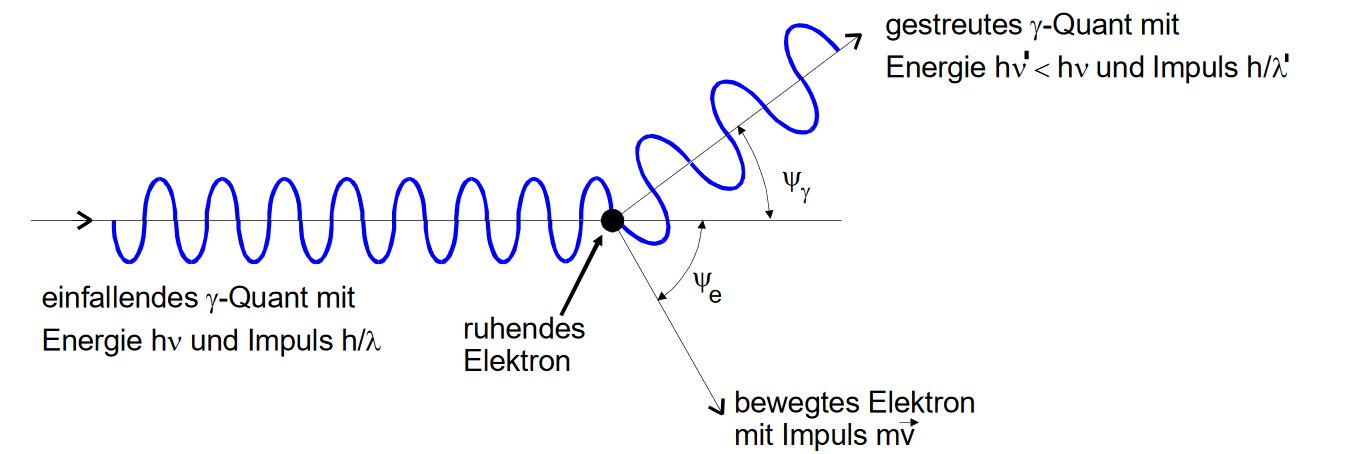
\includegraphics[width=\linewidth,height=\textheight-170pt,keepaspectratio]{content/images/com.png}
	\label{fig:com}
\end{figure}
Für den Wirkungsquerschnitt von der Compton-Streuung gilt
\begin{equation}
\sigma_\text{com} = 2 \pi r_\text{e}^2 \left\{ \frac{1+\epsilon}{\epsilon^2} \left[\frac{2 (1+\epsilon)}{1+2 \epsilon} -\frac{1}{\epsilon} \ln(1+ 2 \epsilon)\right] + \frac{1}{2 \epsilon} \ln(1 + 2 \epsilon) -\frac{1 + 3 \epsilon}{(1+2\epsilon)^2} \right\}
\end{equation}
mit dem klassischen Elektronenradius
\begin{equation}
	r_\text{e} = \frac{e_0^2}{4 \pi \epsilon_0 m_0 c^2} \approx \SI{2.82e-15}{\meter}
\end{equation}
und dem Verhältnis $\epsilon = E_\gamma / (m_0 c^2)$.
Hierin sind $m_0$ die Ruhemasse des Elektrons, $e_0$ die Elementarladung und $\epsilon_0$ die Influenzkonstante. Dieser Ausdruck für $\sigma_\text{com}$ vereinfacht sich für $E_\gamma \ll m_0 c^2$ zu
\begin{equation}
	\sigma_\text{com} \approx \frac{8}{3} \pi r_\text{e}^2 = \sigma_\text{Th} \text{.}
\end{equation}
Dabei wird $\sigma_\text{Th}$ als Thomsonscher Wirkungsquerschnitt bezeichnet.
Für $E_\gamma \gg m_0 c^2$ ist $\sigma_\text{com} \propto 1/\epsilon$. 
Bei der Paarbildung kann ein $\gamma$-Quant ein Elektron und ein Positron erzeugen. Dieser Effekt kann nur auftreten falls die Energie vom $\gamma$-Quant $E_\gamma > 2 m_o c^2$ ist und ein Teil des Impulses auf ein weiteres Teilchen übertragen werden kann. Dabei wird das $\gamma$-Quant annihiliert und die zusätzliche Energie in die kinetische Energie der Teilchen umgewandelt. Aus der Quantentheorie folgt, dass $\sigma_\text{p} \propto z^2$ ist.
Alle Effekte überlagern sich und bilden ein Verlauf von $\sigma$ der insbesondere von $E_\gamma$ abhängt. Für das Material Germanium ist dieser in Abbildung \ref{fig:kurve1} dargestellt.
\begin{figure}
	\centering
	\caption{Darstellung der Abhängigkeit des Absorptionskoeffizienten von der Energie und die Anteile der einzelnen Effekte an diesem für Germanium \cite{V704}.}
	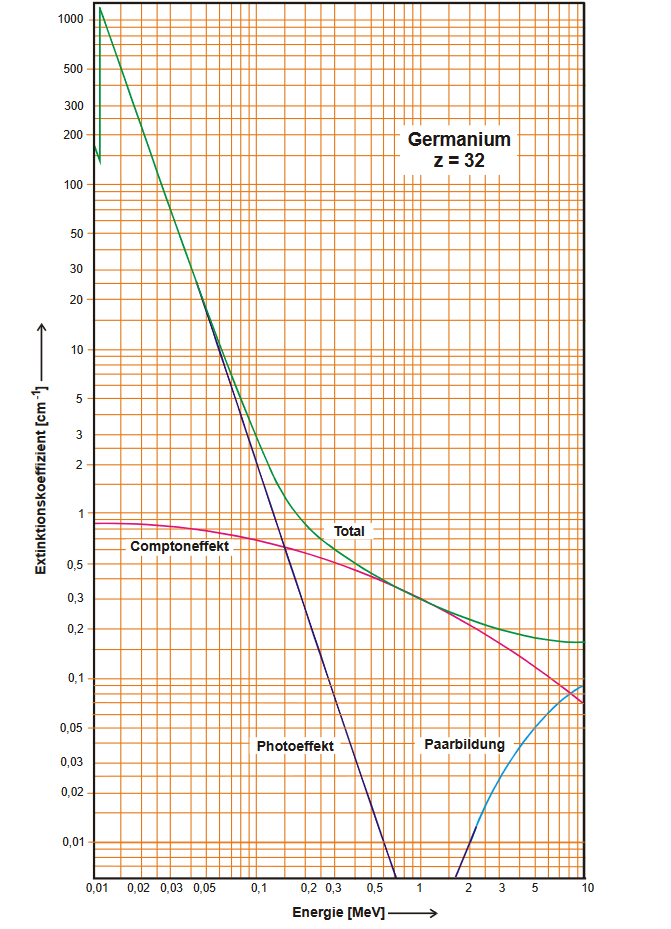
\includegraphics[width=\linewidth-170pt,height=\textheight-170pt,keepaspectratio]{content/images/kurvenverlauf1.png}
	\label{fig:kurve1}
\end{figure}

\subsection{\texorpdfstring{Entstehung und Absorptionsverhalten von $\beta$-Strahlung}{}}
$\beta$-Strahlung besteht aus $\beta$-Teilchen, welche durch Umwandlung eines Nukleons in einem Atomkern erzeugt und danach emittiert werden.
Die Umwandlung des Nukleons folgt entweder dem Reaktionsschema
\begin{equation}
 n \to p + \beta^- +\overline{\nu}_e
\end{equation}
oder 
\begin{equation}
p \to n + \beta^+ +\nu_e\text{.}
\end{equation}
Die dabei freiwerdende Energie $E_\text{f}$ verteilt sich statistisch auf die entstehenden Teilchen, sodass das Energiespektrum kontinuierlich ist. Die maximale Energie die ein $\beta$-Teilchen erhalten kann $E_\text{max}$ entspricht der freiwerdende Energie $E_\text{f}$. Die Verteilung der Energien der $\beta$-Teilchen ist in Abbildung \ref{fig:eSpektrum} dargestellt.
\begin{figure}
	\centering
	\caption{Darstellung des Energiespektrums der $\beta$-Teilchen \cite{V704}.}
	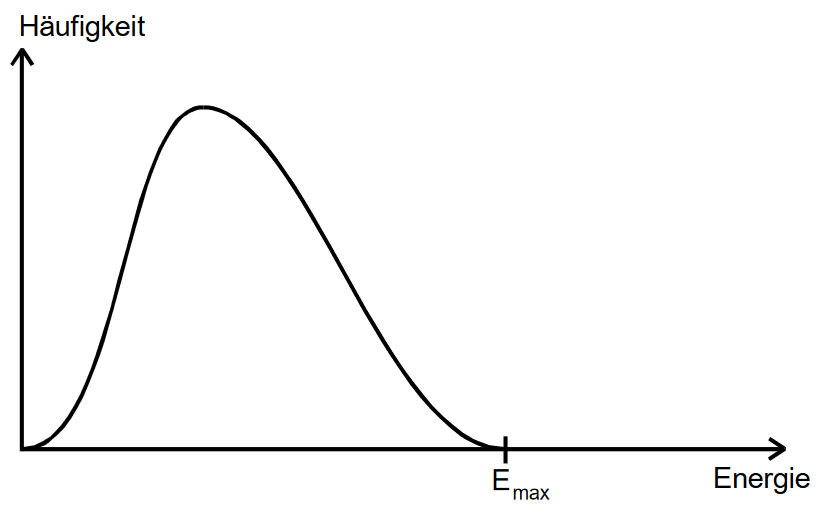
\includegraphics[width=\linewidth-170pt,height=\textheight-170pt,keepaspectratio]{content/images/emissionEnergie.png}
	\label{fig:eSpektrum}
\end{figure}
Die $\beta$-Teilchen werden im Material sowohl elastisch an den Atomkernen als auch inelastisch an den Atomkernen und Elektronen gestreut.
Die elastische Streuung an den Atomkernen führt zu staken Richtungsänderungen und längeren effektiven Wegen der $\beta$-Teilchen im Material, wie in Abbildung \ref{fig:verlaufTeilchen} dargestellt ist.
\begin{figure}
	\centering
	\caption{Beispielhafte Wege von einzelnen $\beta$-Teilchen in Materie \cite{V704}.}
	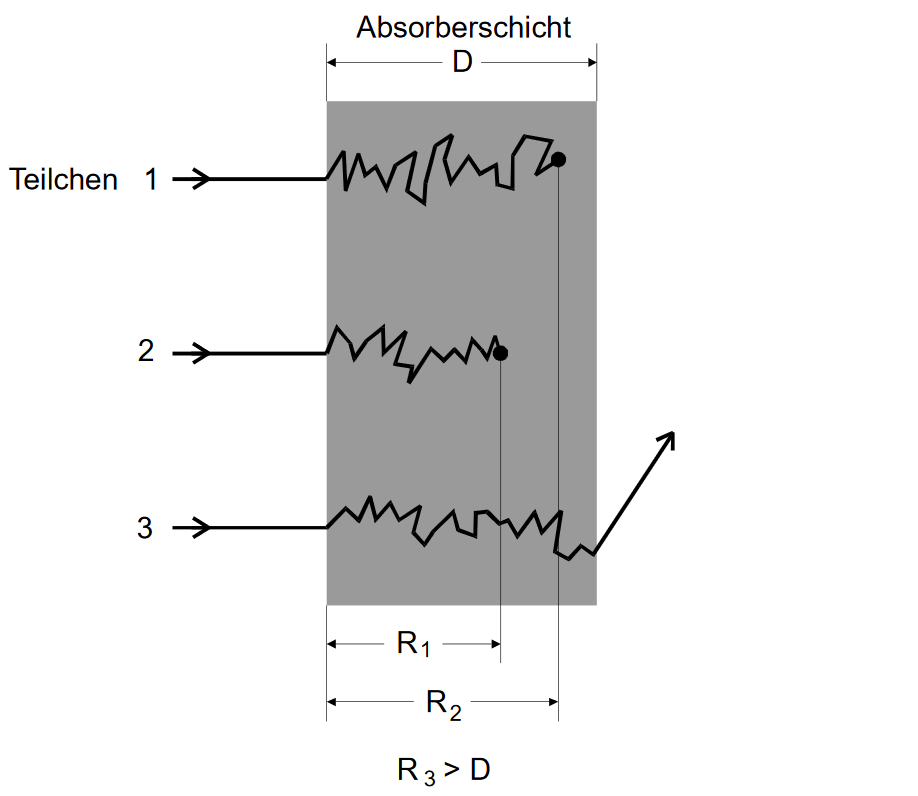
\includegraphics[width=\linewidth-170pt,height=\textheight-170pt,keepaspectratio]{content/images/verlaufTeilchen.png}
	\label{fig:verlaufTeilchen}
\end{figure}
Die inelastische Streuung an den Atomkernen tritt auf wenn sich die geladenen $\beta$-Teilchen durch die elektrischen Felder der Kerne bewegen und dadurch beschleunigt werden. Bei der Beschleunigung von geladenen Teilchen werden jedoch elektromagnetische Wellen abgestrahlt, was zu einem Energieverlust der Teilchen führt. Die enstehende Strahlung wird als Bremsstrahlung bezeichnet. Die Wahrscheinlichkeit, dass Bremsstrahlung auftritt ist durch den Wirkungsquerschnitt
\begin{equation}
\sigma_\text{Br}=\alpha r_\text{e}^2 z^2
\end{equation}
gegeben, wobei $\alpha\approx 1/137$ die Sommerfeldsche Feinstruckturkonstante ist. Für den mittleren Energieverlust einer $\beta$-Teilchen mit der Energie $E_\beta$ gilt
\begin{equation}
\overline{E_\text{Br}} \approx 7 10^{-7} z E_\beta^2 \text{.}
\end{equation}
Diese Näherung ist gültig für Energien bis etwa $\SI{2500}{\kilo\electronvolt}$.
Die Wahrscheinlichkeit einer inelastische Streuung der $\beta$-Teilchen durch Ionisation oder Anregung der Atome im Absorber wächst mit der Anzahl der Elektronen pro Volumen an. Dabei geben die $\beta$-Teilchen jeweils nur einen kleinen Teil ihrer Energie ab. Der Energieverlust der $\beta$-Teilchen pro Absorberschichtdicke ist für $\beta$-Teilchen mit $E_\beta < m_0 c^2$ durch
\begin{equation}
\frac{\diff E}{\diff x} \approx - \frac{2 \pi r_\text{e}^2}{E_\beta} \frac{N_\text{L} \rho}{M} z \ln\left(\frac{E_\beta}{I}\right)
\end{equation}
gegeben, wobei $I$ die Ionisierungsenergie ist.

Für die Absorbtionskurve von $\beta$-Strahlung eines natürlichen Strahlers ergibt sich eine Kurve der in Abbildung \ref{fig:kurvenverlauf2} dargestellten Form, wobei statt der Schichtdicke $D$ des Absorbers die Massenbelegung $R = \rho D$ aufgetragen ist. Aus dieser Absorptionskurve kann durch Näherung der linearen Anteile und Bestimmung des Schnittpunktes die maximale Reichweite $R_\text{max}$ der $\beta$-Teilchen bestimmt werden. Diese hängt mit der maximalen Energie der $\beta$-Teilchen $E_\text{max}$ zusammen. Im für den Versuch bedeutsamen Energiebereich gilt der Zusammenhang
\begin{equation}
	E_\text{max}=1.92 \sqrt{R_\text{max}^2 + 0.22 R_\text{max}}\text{ ,}\label{eq:HJKH}
\end{equation}
wobei $E_\text{max}$ in $\si{\mega\electronvolt}$ und $R_\text{max}$ in $\si{\gram\per\centi\meter\squared}$ ist.
Der Zusammenhang wurde empirisch bestimmt.









\begin{figure}
	\centering
	\caption{Absorptionskurve von $\beta$-Teilchen in Materie \cite{V704}.}
	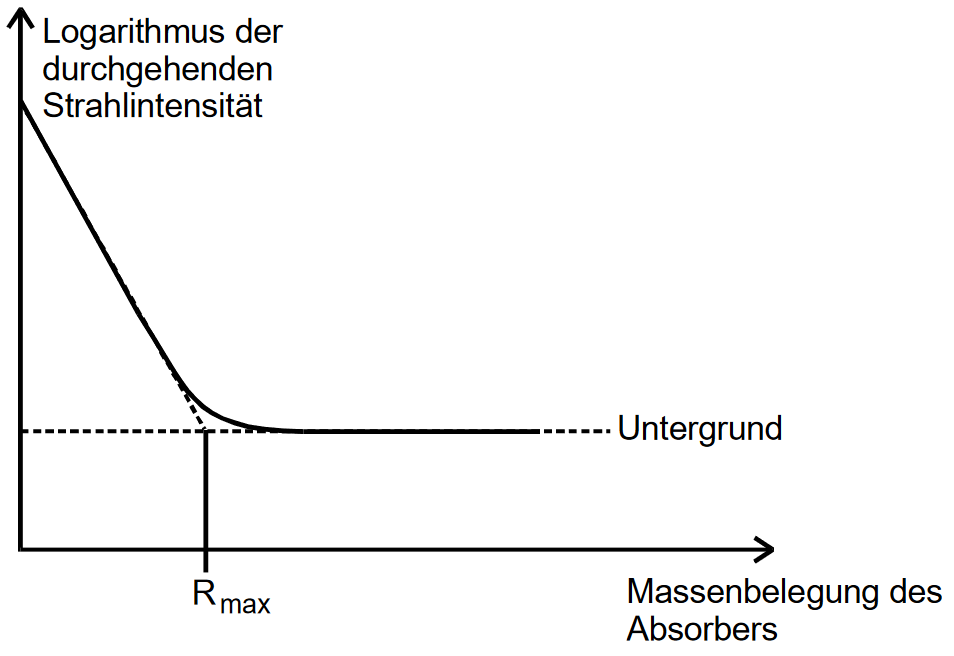
\includegraphics[width=\linewidth-170pt,height=\textheight-170pt,keepaspectratio]{content/images/kurvenverlauf2.png}
	\label{fig:kurvenverlauf2}
\end{figure}




